\documentclass{ximera}

\newcommand{\RR}{\mathbb R}
\renewcommand{\d}{\,d}
\newcommand{\dd}[2][]{\frac{d #1}{d #2}}
\renewcommand{\l}{\ell}
\newcommand{\ddx}{\frac{d}{dx}}
\newcommand{\dfn}{\textbf}
\newcommand{\eval}[1]{\bigg[ #1 \bigg]}


\outcome{Solve basic related rates word problems.}
\outcome{Understand the process of solving related rates problems.}
\outcome{Calculate derivatives of expressions with multiple variables implicitly.}

\title[Dig-In:]{More than one rate}

\begin{document}
\begin{abstract}
  Here we work abstract related rates problems.
\end{abstract}
\maketitle


Suppose we have two variables $x$ and $y$ which are both changing with
respect to time.  A \textit{related rates} problem is a problem where
we know one rate at a given instant, and wish to find the other (the unknown rate is "related" to the known rate).

Here the chain rule is key: If $y$ is written in terms of $x$, and we
are given $\dd[x]{t}$, then it is easy to find $\dd[y]{t}$ using the
chain rule:
\[
y=y(x)
\]
\[
\dd[y]{t}=y'(x(t))\cdot x'(t).
\]
In many cases, particularly the interesting ones, our functions will
be related in some other way. Nevertheless, in each case we'll use the
power of the chain rule to help us find the desired rate. In this
section, we will work several abstract examples, so we can emphasize
the mathematical concepts involved. In each of the examples below, we
will follow essentially the same plan of attack:



\begin{description}
\item[\textbf{Introduce variables, identify the given and unknown rates.}] Assign a variable to each quantity that changes in time.
\item[\textbf{Draw a picture.}] If possible, draw a schematic picture with all the relevant information. 
\item[\textbf{Find equations.}] Write equations that relate all
  relevant variables.
\item[\textbf{Differentiate with respect to t.}] Here we will often use
  implicit differentiation and obtain an equation that relates the given rate and the unknown rate. 
\item[\textbf{Evaluate and solve.}] Evaluate
each quantity at the relevant instant and solve for the unknown rate.

\end{description}




\section{Formulas}

In order to relate several variables we can use known formulas.

In our next example we consider an expanding circle and use the formulas for perimeter and area of a circle.

    \begin{image}
      \begin{tikzpicture}
       width=2in,
        height=2in
        \draw [penColor,thick] (0,0) circle [radius=0.5];
           \draw [penColor, dashed] (0,0) circle [radius=0.8];
             \draw [penColor, dashed] (0,0) circle [radius=1.1];
            
      \end{tikzpicture}
    \end{image}
\begin{example}
  Imagine an expanding circle. If we know that the perimeter is
  expanding at a rate of $4$ m/s, at what rate is the area changing
  when the radius is $3$ meters?
  \begin{explanation}
  
 

   First, we \textbf{introduce the variables} $P$, $r$, and $A$,  denoting the perimeter, the radius, and  the area of the circle, in that order. 
   
   We \textbf{identify} the given rate, $\frac{dP}{dt}=4$ m/s, and the unknown rate, $\Bigl[\frac{dA}{dt}\Bigr]_{r=3}$, the rate to be determined. 
   
    Next, we \textbf{draw a picture}.
    \begin{image}
      \begin{tikzpicture}
        \draw [penColor, very thick] (0,0) circle [radius=2];
        \draw [penColor] (0,0) -- (2,0);
        \node [below,penColor] at (1,0) {$r$ };
        \node [penColor,left] at (-1.65,1.42) {$\dfrac{d}{dt}P(t) = 4$ m/s};
        \node [penColor,left] at (-2.1,0.2) {$\Bigl[\frac{dA}{dt}\Bigr]_{r=3} = $ ? };
        
      \end{tikzpicture}
    \end{image}
   Now we have to \textbf{find equations} that relate
   the variables $P$, $r$, and $A$. 
   
   Naturally, we think of formulas for perimeter and area of a circle
    \[
    P = 2\cdot \pi \cdot \answer[given]{r}
    \qquad\text{and}\qquad
    A = \pi \cdot \answer[given]{r^{2}}.
    \]
   We know that the perimeter of the circle is expanding. This implies that both the radius and the area of the circle are changing in time, too.
    So, we note that $P$, $r$, and $A$ are functions of time
    \[
    P(t) = 2\cdot \pi \cdot r(t)
    \qquad\text{and}\qquad
    A(t) = \pi \cdot r(t)^2.
    \]
    We \textbf{differentiate} both sides of each equation with respect to time, $t$.  Using implicit
    differentiation, we get that
    
    \[
  \underbrace{ \dfrac{d}{dt}P(t)}_{given\hspace{0.05in} rate} = 2\cdot \pi\cdot  \dfrac{d}{dt}r(t)
    \qquad\text{and}\qquad
    \underbrace{ \dfrac{d}{dt}A(t)}_{unknown \hspace{0.05in}rate} = 2\cdot \pi\cdot r(t) \cdot  \dfrac{d}{dt}r(t).
    \]
    
    These two equations hold on some time interval. In particular, they are both true at an instant when $r=3$.
    
   We know  that at that instant $\Bigl[ \dfrac{d}{dt}P(t)\Bigr]_{r=3} =
    \answer[given]{4}$ and $r = \answer[given]{3}$. 
    
    Using this, we \textbf{evaluate}  the two equations at the instant when $r=3$.
    
        \[
    4 = 2\cdot \pi\cdot \Bigl[\dfrac{d}{dt}r(t)\Bigr]_{r=3}
    \qquad\text{and}\qquad
   \Bigl[ \dfrac{d}{dt}A(t)\Bigr]_{r=3} = 2\cdot \pi\cdot 3 \cdot \Bigl[\dfrac{d}{dt}r(t)  \Bigl]_{r=3}.
    \]
    
    
   From the first equation we get that
    \begin{align*}
      \Bigl[\dfrac{d}{dt}r(t)\Bigr]_{r=3}&=  2/\pi \hspace{0.1in} m/s.    
    \end{align*} 
   
  Using this result and the equation on the right, we get that
   
    \begin{align*}
     \Bigl[ \dfrac{d}{dt}A(t)\Bigr]_{r=3} &= 2\cdot \pi\cdot 3 \cdot 2/\pi\\
      &=\answer[given]{12}\hspace{0.1in} m^2/s.
    \end{align*}
    Hence, the area is expanding at a rate of $12$ $m^2/s$ at the instant when $r=3$ m.
  \end{explanation}
\end{example}


%%BADBAD
%% There are a number of common formulas that arise in related rates
%% problems.
%%
%% It might be nice to add a little list of common area/volume formulas.



\section{Right triangles}


In our next example we consider an expanding right triangle and use the Pythagorean Theorem to relate relevant variables.
 \begin{image}
      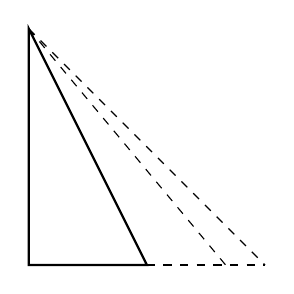
\begin{tikzpicture}
         \coordinate (A) at (0,0);
        \coordinate (B) at (0,3);
        \coordinate (C) at (1.5,0);
        \coordinate (D) at (2.5,0);
         \coordinate (E) at (3,0);
        \tkzMarkRightAngle(C,A,B)
        \tkzDefMidPoint(A,B) \tkzGetPoint{3 m}
        \tkzDefMidPoint(A,C) \tkzGetPoint{b}
        \tkzDefMidPoint(B,C) \tkzGetPoint{c}
        \draw [thick](A)--(B)--(C)--cycle;
         \draw[dashed](B)--(D);
          \draw[dashed](B)--(E);
          \draw[dashed](C)--(E);
           \tkzLabelPoints[left](3 m)
        %\tkzLabelPoints[left](a)
      
      \end{tikzpicture}
    \end{image}

\begin{example}
  Imagine an expanding right triangle. If one leg has a fixed length
  of $3$ m, one leg is increasing with a rate of $2$ m/s, and the
  hypotenuse is expanding to accommodate the expanding leg, at what
  rate is the hypotenuse expanding when both legs are $3$ m long?
  \begin{explanation}
 First, we \textbf{introduce the variables}  $a$, $b$, and $c$, denoting the fixed length, the length of a leg that is increasing, 
 and  the length of the hypotenuse, in that order. Then, we \textbf{identify} the given rate $\frac{db}{dt}=2$ m/s and the unknown rate $\Bigl[\frac{dc}{dt}\Bigr]_{b=3}$, the rate to be determined.
   Now, we \textbf{draw a picture}.
    \begin{image}
      \begin{tikzpicture}
         \coordinate (A) at (0,0);
        \coordinate (B) at (0,3);
        \coordinate (C) at (1.5,0);
        \tkzMarkRightAngle(C,A,B)
        \tkzDefMidPoint(A,B) \tkzGetPoint{a}
        \tkzDefMidPoint(A,C) \tkzGetPoint{b}
        \tkzDefMidPoint(B,C) \tkzGetPoint{c}
        \draw (A)--(B)--(C)--cycle;
        \tkzLabelPoints[right](c)
        \tkzLabelPoints[above](b)
     
        %\tkzLabelPoints[left](a)
        \node [left] at (a) {$a = 3m$};
      \node [penColor] at (2.4,2.42){$\frac{db}{dt} = 2$};
        \node [penColor,left] at (3.9,1.25) {$\Bigl[\frac{dc}{dt}\Bigr]_{b=3} = $ ? };
      \end{tikzpicture}
    \end{image}

    Next, we  \textbf{find equations} that relate relevant
    variables. Here we use the Pythagorean Theorem.
    \[
    c^2 = a^2 + b^2
    \]
   Note that $a=3$ is a constant, and $c$ and $b$ are functions of time, $t$.
    We, then, \textbf{differentiate} both sides of the equation with respect to $t$,  using  implicit differentiation
  
       \[
    2\cdot c\cdot \dfrac{dc}{dt} = 2\cdot b\cdot \dfrac{db}{dt}.
    \]
    Now, we \textbf{evaluate} all the quantities at the instant when $b=3$, noting that
    $\Bigl[\dfrac{db}{dt}\Bigr]_{b=3} = 2$ and that $b = 3$. Therefore,
    \[
    2\cdot [c]_{b=3}\cdot \Bigl[\dfrac{dc}{dt}\Bigr]_{b=3} = \answer[given]{12}.
    \]
    We need to compute $[c]_{b=3}$, the length of the hypotenuse at the instant when $b=3$. Here we use
    the Pythagorean Theorem
    \begin{align*}
    \Bigl([c]_{b=3}\Bigr)^2 &= 3^2 + 3^2\\
    &=\answer[given]{18},
    \end{align*}
    So, we see that $[c]_{b=3} = 3\sqrt{2}$. \\
    Then, we \textbf{solve} for the rate.\\
    \begin{align*}
      6\sqrt{2}\cdot \Bigl[\dfrac{dc}{dt}\Bigr]_{b=3} &= 12 \\     
      \Bigl[\dfrac{dc}{dt}\Bigr]_{b=3} &= \sqrt{2}.
    \end{align*}
    Therefore, the hypotenuse  is growing at a rate of $\answer[given]{\sqrt{2}}$ m/s when both legs are $3m$ long.
  \end{explanation}
\end{example}


\section{Angular rates}


We can also investigate problems involving angular rates.

\begin{example}
  Imagine an expanding right triangle. If one leg has a fixed length
  of $3$ m, one leg is increasing with a rate of $2$ m/s, and the
  hypotenuse is expanding to accommodate the expanding leg, at what
  rate is the angle opposite the fixed leg changing when both legs
  are $3$ m long?
  \begin{explanation}
  First, we \textbf{introduce the variables}  $a$, $b$, $c$, and $\theta$, denoting the fixed length, the length of a leg that is increasing, 
  the length of the hypotenuse, and the angle opposite the leg with fixed length,  in that order. 
  
  
  We \textbf{identify} the given rate $\frac{db}{dt}=2$ m/s and the unknown rate $\Bigl[\frac{d\theta}{dt}\Bigr]_{b=3}$, the rate to be determined.
  
  
    Next, we \textbf{draw a picture}.
    \begin{image}
      \begin{tikzpicture}
        \coordinate (A) at (0,2);
        \coordinate (B) at (0,5);
        \coordinate (C) at (6.5,2);
        \tkzMarkRightAngle(C,A,B)
        \tkzMarkAngle[size=1.2cm,thin](B,C,A)
        \tkzLabelAngle[pos = 1](B,C,A){$\theta$}
        \tkzDefMidPoint(A,B) \tkzGetPoint{a}
        \tkzDefMidPoint(A,C) \tkzGetPoint{b}
        \tkzDefMidPoint(B,C) \tkzGetPoint{c}
        \draw (A)--(B)--(C)--cycle;
        \tkzLabelPoints[above](c)
        \tkzLabelPoints[above](b)
        %\tkzLabelPoints[left](a)
        \node [left] at (a) {$a = 3$};
       \node [penColor,left] at (3.1,1.2){$\frac{db}{dt} = 2$};
        \node [penColor,left] at (6.1,1.2) {$\Bigl[\frac{d\theta}{dt}\Bigr]_{b=3} = $ ? };
      \end{tikzpicture}
    \end{image} 

    We now \textbf{find equations} that combine relevant
    variables. Here we note that
    \[
    \tan(\theta) = \frac{a}{\answer[given]{b}}.
    \]
    Since $\theta$ and $b$ are functions of time, we
      \textbf{differentiate}  both sides of  the equation using
    implicit differentiation.
  (Note: $a$ is constant).
    \[
    \sec^2(\theta)\frac{d\theta}{dt} = \frac{-a}{b^2}\cdot \frac{db}{dt}.
    \]
    Now, we \textbf{evaluate} all the quantities at the instant when $b=3$, keeping in mind that
     $a=3$, $\frac{db}{dt} = 2$, and $b = 3$.
    \begin{align*}
    \Bigl[\sec^2(\theta)\Bigr]_{b=3}\cdot \Bigl[\dfrac{d\theta}{dt}\Bigr]_{b=3} &= \frac{-3\cdot 2}{3^2}\\
    &= \frac{-2}{3}.
    \end{align*}
    However, we still need to compute $ \Bigl[\sec^2(\theta)\Bigr]_{b=3}$. Here we use a trig identity
  
    \begin{align*}
     \Bigl[\sec^2(\theta)\Bigr]_{b=3} &= 1+ \Bigl[\tan^2(\theta)\Bigr]_{b=3}\\
      &= 1+\Bigl(\frac{3}{3}\Bigr)^2\\
      &= \answer[given]{2}.
    \end{align*}
   Now we \textbf{solve}.
    \begin{align*}
      2\cdot \Bigl[\dfrac{d\theta}{dt}\Bigr]_{b=3}  &= \frac{-2}{3}\\
     \Bigl[\dfrac{d\theta}{dt}\Bigr]_{b=3} &= \frac{-1}{3}.
    \end{align*}
    So, when $b=3$, the angle is changing at $\answer[given]{-1/3}$
    radians per second.
  \end{explanation}
\end{example}



\section{Similar triangles}

Finally, facts about similar triangles are often useful when solving
related rates problems.

\begin{example}
  Imagine two right triangles that share an angle:
  \begin{image}
    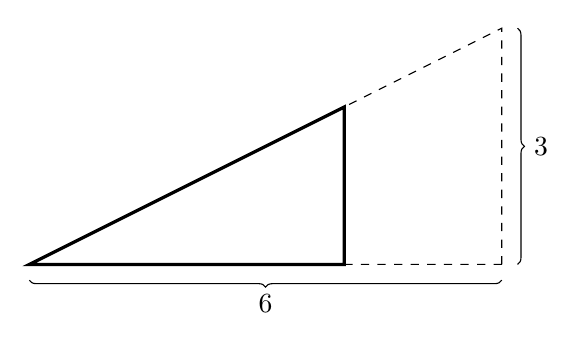
\begin{tikzpicture}
      \coordinate (A) at (6,2);
      \coordinate (B) at (6,5);
      \coordinate (C) at (0,2);
      \coordinate (D) at (4,2);
      \coordinate (E) at (4,4);
      \tkzMarkRightAngle(C,A,B)
      \tkzMarkRightAngle(C,D,E)
      \tkzDefMidPoint(A,B) \tkzGetPoint{a}
      \tkzDefMidPoint(A,C) \tkzGetPoint{b}
      \tkzDefMidPoint(D,C) \tkzGetPoint{x}
      \draw[decoration={brace,mirror,raise=.2cm},decorate,thin] (0,2)--(6,2);
      \draw[decoration={brace,mirror,raise=.2cm},decorate,thin] (6,2)--(6,5);
      \draw[dashed] (A)--(B)--(C)--cycle;
      \draw[very thick] (D)--(E)--(C)--cycle;
      \tkzLabelPoints[above](x)
      \node at (3,2-.5) {$6$};
      \node at (6+.5,3.5) {$3$};
    \end{tikzpicture}
  \end{image}
  If $x$ is growing from the vertex with a rate of $3$ m/s, what rate
  is the area of the smaller triangle changing when $x = 5$m?
  \begin{explanation}
  First, we \textbf{introduce the variables} $h$, the height of the smaller triangle, and $A$, the area of the smaller triangle.
Next, we \textbf{identify} the given rate $\frac{dx}{dt}=3$ m/s and the unknown rate $\Bigl[\frac{dA}{dt}\Bigr]_{x=5}$, the rate to be determined.
    Despite the fact that a nice picture is given, we should do what
    we always do and \textbf{draw a picture}. Note, we ad
    information to the picture:
    \begin{image}
      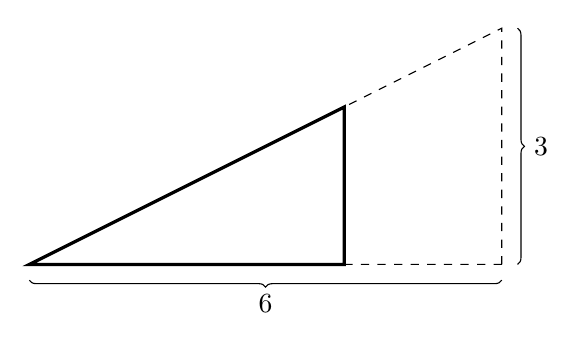
\begin{tikzpicture}
        \coordinate (A) at (6,2);
        \coordinate (B) at (6,5);
        \coordinate (C) at (0,2);
        \coordinate (D) at (4,2);
        \coordinate (E) at (4,4);
        \tkzMarkRightAngle(C,A,B)
        \tkzMarkRightAngle(C,D,E)
      \tkzDefMidPoint(A,B) \tkzGetPoint{a}
      \tkzDefMidPoint(A,C) \tkzGetPoint{b}
      \tkzDefMidPoint(D,C) \tkzGetPoint{x}
      \tkzDefMidPoint(D,E) \tkzGetPoint{h}
      \draw[decoration={brace,mirror,raise=.2cm},decorate,thin] (0,2)--(6,2);
      \draw[decoration={brace,mirror,raise=.2cm},decorate,thin] (6,2)--(6,5);
      \draw[dashed] (A)--(B)--(C)--cycle;
      \draw[very thick] (D)--(E)--(C)--cycle;
      \tkzLabelPoints[above](x)
      \tkzLabelPoints[right](h)
      \node at (3,2-.5) {$6$};
      \node at (6+.5,3.5) {$3$};
    \end{tikzpicture}
  \end{image}


    Next, we \textbf{find equations} that combine relevant
    variables. In this case there are two. The first is the formula
    for the area of a triangle:
    \[
    A = \answer[given]{(1/2) \cdot x \cdot h}
    \]
    The second uses the fact that the larger triangle is similar to
    the smaller triangle, meaning that the ratios between the corresponding sides in both triangles
    are equal,
    \[
    \frac{x}{h} = \answer[given]{\frac{6}{3}}\qquad\text{so}\qquad x =
    \answer[given]{2}\cdot h
    \]
   Since $A$, $x$, and $h$ are functions of time, we write
    \[
    A(t) = (1/2) \cdot x(t) \cdot h(t) \qquad\text{and}\qquad x(t) =
    2\cdot h(t).
    \]
    We now  \textbf{differentiate} both sides of each equation using
    implicit differentiation, treating all functions as functions of
    $t$,
    \begin{align*}
    \dfrac{d}{dt}A(t) &= (1/2) \cdot\dfrac{d}{dt}x(t) \cdot h(t) +  (1/2) \cdot x(t) \cdot \dfrac{d}{dt}h(t),\\
     \dfrac{d}{dt}x(t) &= 2\cdot\dfrac{d}{dt}h(t)
    \end{align*}
    Now we \textbf{evaluate} all the quantities at the moment when $x=5$m.
    \[
    5 = 2\cdot [h(t)]_{x=5}\qquad\text{and}\qquad 3= 2\cdot \Bigl[\dfrac{d}{dt}h(t)\Bigr]_{x=5}
    \]
    we see that $ [h(t)]_{x=5} = 5/2$ and $ \Bigl[\dfrac{d}{dt}h(t)\Bigr]_{x=5} = 3/2$. \\
    Now we \textbf{solve} for the rate.
    \begin{align*}
    \Bigl[\dfrac{d}{dt}A(t)\Bigr]_{x=5}  &= (1/2) \cdot 3 \cdot (5/2) + (1/2) \cdot 5 \cdot (3/2)\\
      &= 15/4 + 15/4\\
      &= \answer[given]{15/2}.
    \end{align*}
    Hence, the area is changing at a rate of $15/2$ $\text{m}^2/\text{s}$ when $x=5$m.
    
  \end{explanation}
\end{example}
\end{document}
